\pagebreak
\question
Die häufigste Speichertechnologie
für den Arbeitsspeicher
sind aktuell noch DRAMs. Ein Nachteil der DRAM-Technologie ist u.\,a. der häufig erforderliche Refresh.

Zeigen Sie anhand der beigefügten schematischen Skizze einer einzelnen DRAM-Zelle, warum ein Refresh erforderlich ist und wie dieser abläuft.
\begin{solutionordottedlines}[2cm]
\begin{center}
	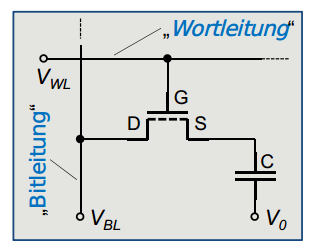
\includegraphics[width=\linewidth]{Refresh_Reason.png}
\end{center}
\begin{description}
	\item [Ursache]
	Zwischen S (Source) und D (Drain) kommt es aufgrund von Verunreinigungen zum Stromfluss.
	Ein gespeicherter Wert in C kann dadurch ungewollt abfliessen (oder sich auffüllen).
	\item[Ablauf Refresh]
	Bei einem Refresh, der alle paar 100 ns passiert, wird jeder Wert gelesen und gleich wieder geschrieben. Auf diese Weise ist die Ladung (oder nicht-Ladung) ständig in ihrer Position gehalten. Es ist gewissermassen so, als hätte man ein paar Krabbeltiere in einem offenen Glas und würde ständig die, die flüchten, wieder zurückschieben, oder die, die ungewollt hinein kriechen, wieder entfernen. 
\end{description}
Anmerkung: Skizze aus Skript entlehnt.
\end{solutionordottedlines}
